\section{Approach}
In this section, we discuss the detailed process of problem formulation, including the relevant model objective and assumptions, and the definition of elements in our proposed multi-agent reinforcement learning model for collision avoidance. Besides, we present our proposed algorithm framework and related environment settings in our simulation experiments.

\subsection{Modeling}
The objective in our case studies is to ensure sufficient safe separation and avoid collision between aircrafts by providing speed advisories. The agents needs to learn and coordinate to maintain safe separation at every time step under stochastic and dynamic environment. Since our experiments are implemented on the Bluesky simulator, performance metrics assumptions related to different aircraft type and flight rules are predefined. Here we indroduce thorough formulation of the D2MARL problem by representing each aircraft as an agent and defining the corresponding state space, action space, termniation criteria and reward function.

\subsubsection{State Space}
The state information for the ownship contains the distance to the target, speed, speed change, direction variation, route identifier and the loss of separation distance. For the intruders, except the corresponding information for the ownship, their state space also concludes the mutual distance among ownship, intersection and the intruder self. An intersection plays a important part in defining a potential conflict between the ownship and intruders. Thus, we make the following assumptions that aircraft, which is either on the same route or in the conflicting route, must not have reached the intersection on conflicting route. 

Specifically, the state information for the ownership and the intruder are given respectively as follows:


$$s_t^o = \left( {d_{{\rm{goal}}}^{(o)},{v^{(o)}},{a^{(o)}},{d_l^{(o)}},{r^{(o)}},LOS} \right)$$

$$h_t^o\left( i \right) = \left( {d_{{\rm{goal}}}^{(i)},{v^{(i)}},{a^{(i)}},{d_l^{(i)}},{r^{(i)}},d_o^{(i)},d_{{\mathop{\rm int}} }^{(o)},d_{{\mathop{\rm int}} }^{(i)}} \right)$$

As listed above, the state at time $t$ consists of two part, the ownship state $s_t^o$ and the state of intruders $h_t^o$ that is available to the ownship. Here we explain the symbols in the state. Note that we don't put ownership's distance to the intersection into the ownership state, since one aircraft might encounter more than one intersection, and the dimension of the state can not be fixed then. Therefore, we can put such information into the intruders' state so that every intruder will have one and only one term of $d_{int}^{(o)}$ will be added, while $d_{int}^{(o)}$ is for the \textit{i-th} intruder's distance to the intersection. $d_{goal}^{(o)}$ and $d_{goal}^{(i)}$ descrbie the ownership's and the \textit{i-th} intruder's distance to the its goal. Similarly, to discribe other state information of the ownership and the \textit{i-th} intruder, we use $v$ for the velocity, $a$ for the last action taken, $d_l$ for the distance away from the airline, and $r$ for the airplane's radius which is useful for checking collisions. The $LOS$ value could varies depending on the aircraft type, but here we keep it the same just as supplementary information. $d_o^{(i)}$ describes the distance between the ownership and the \textit{i-th} intruder. Figure \ref{fig:intersect} and Figure \ref{fig:airway} explain the setting of the state space.

\subsubsection{Action Space}
The action space here could change according to our experiment settings. An action could be described as "to change the speed" or "to change the direction". To make the action space more complex, it could be described as "to change both of them", that is, "to change the velocity". More details are shown in Section \ref{sec:experiment}, the experiment part.

\subsubsection{Terminal State}
In each episode, a certain number of aircraft will be generated and the current state will come to an end if the following conditions are satisfied:

\[{N_{aircraft}} = 0\]

\subsubsection{Reward Function}
For any agent, the rewrad funtion are the same but the cooperation between the agents are encouraged. More precisely, if two agents are in a collision, they will receive a penalty. We define confict as the distance between two agents is less than 3 nautical miles, that is ${d^{LOS}} = 3$. Besides, the reward function is designed for the agents:

\[{r_t} = \left\{ {\begin{array}{*{20}{l}}
    { - 1}&{\rm{ if } \ d_o^c < 3 \ \rm{ or } \ |d^{(o)}_l| > r_a }\\
    { - \alpha  + \beta  \cdot d_o^c}&{\rm{ if } \ d_o^c < 10 \ \rm{ and } \ d_o^c \ge 3}\\
    0&{{\rm{ otherwise }}}
    \end{array}} \right.\]

Where $d_o^c$ is the distance between the ownship and the closest aircraft in nautical miles. $\alpha $ and $\beta $ are the penalty parameters for losing safe separation. By definition, the agents will learn to choose suitable action to maintain the distance requirements. If the $d_o^c < 3$ is violated, it indicates the loss of separation. Note that $d_l^{(o)}$ refers to the distance from the ownership plane to the airline, and $r_a$ refers to the maximum distance that is allowed to be away from the airline. The $|d^{(o)}_l| > r_a$ inequation is considered when direction changes are allowed in the action space. Figure \ref{fig:action} describes the settings for possible actions.

\begin{figure}[!htbp]
    \centering
    \subfigure[\label{fig:intersect}Intersection in a Sector]{
        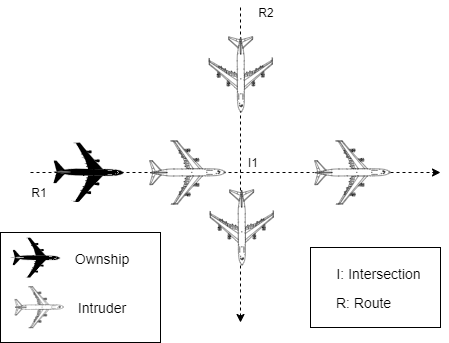
\includegraphics[width=0.3\columnwidth]{images/intersect.png}
    }
    \subfigure[\label{fig:airway}Airline and Airway]{
        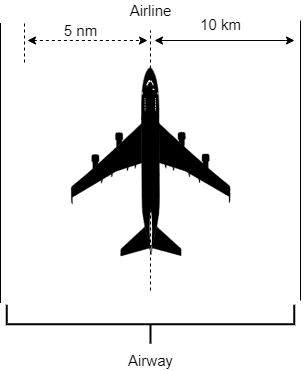
\includegraphics[width=0.18\columnwidth]{images/airway.png}
    }
    \subfigure[\label{fig:action}Possible Actions]{
        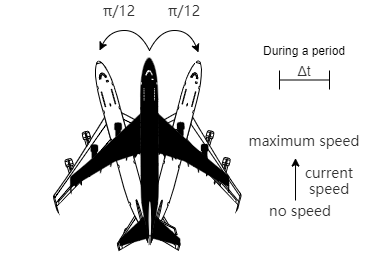
\includegraphics[width=0.3\columnwidth]{images/action.png}
    }
    \caption{State and Action Settings}
    \label{fig:state_action}
\end{figure}


\subsection{Algorithm}
Reinforcement learning can be briefly divided into model-based and model-free methodologies while model-free reinforcement learning can be further classified into value-based and policy-based algorithm. Considering the dynamics in state transition of aircraft movements is hard to determine, and policy-based algorithm is capable to learn stochastic policies where policy gradient direction can increase the possibility of better-than-average actions, we choose Proximal Policy Optimization (PPO) \citep{schulman2017proximal}, a recent policy-based algorithm that uses a neural network to approximate both the policy and the value function, as our basic algorithm framework. The alogorithm process is constructed as below: 
\begin{algorithm}[H]
    \caption{PPO-Clip}
    \begin{algorithmic}[1]
        \REQUIRE
        initial policy parameters $\theta_{0}$, initial value function parameters $\phi_{0}$
        
        \textbf{for} $k=0,1,2, \ldots$ do
        
        1. Collect set of trajectories $\mathcal{D}_{k}=\left\{\tau_{i}\right\}$ by running policy $\pi_{k}=\pi\left(\theta_{k}\right)$ in the environment.

        2. Compute rewards-to-go $\hat{R}_{t}$

        3. Compute advantage estimates, $\hat{A}_{t}$ based on the current value function $V_{\phi_{k}}$.

        4. Update the policy by maximizing the PPO-Clip objective via stochastic gradient ascent with Adam:
$$
\theta_{k+1}=\arg \max _{\theta} \frac{1}{\left|\mathcal{D}_{k}\right| T} \sum_{\tau \in \mathcal{D}_{k}} \sum_{t=0}^{T} \min \left(\frac{\pi_{\theta}\left(a_{t} \mid s_{t}\right)}{\pi_{\theta_{k}}\left(a_{t} \mid s_{t}\right)} A^{\pi_{\theta_{k}}}\left(s_{t}, a_{t}\right), \quad g\left(\epsilon, A^{\pi_{\theta_{k}}}\left(s_{t}, a_{t}\right)\right)\right)
$$

5. Fit value function by regression on mean-squared error via gradient descent algorithm:
$$
\phi_{k+1}=\arg \min _{\phi} \frac{1}{\left|\mathcal{D}_{k}\right| T} \sum_{\tau \in \mathcal{D}_{k}} \sum_{t=0}^{T}\left(V_{\phi}\left(s_{t}\right)-\hat{R}_{t}\right)^{2}
$$

\textbf{end for}   
    \end{algorithmic}
\end{algorithm}
We also consider multi-agent reinforcement learning, where a set of agents share the same environment, as presented in \ref{fig:multi_agent}.The difficulty for an agent lie in how to tackle the relationship between the environments and other agents to obtain a higher reward. In our paper, a centralized learning and decentralized execution framework is introduced. In this way, agents can be trained simultaneously by applying a centralized method where communication is encouraged to implement. It shows that centralized learning can improve the agents' learning efficency while decentralized schemes have an advantage under partial observability and in limited communications during execution \citep{foerster2017counterfactual}.

\begin{figure*}[htbp]
    \centering
    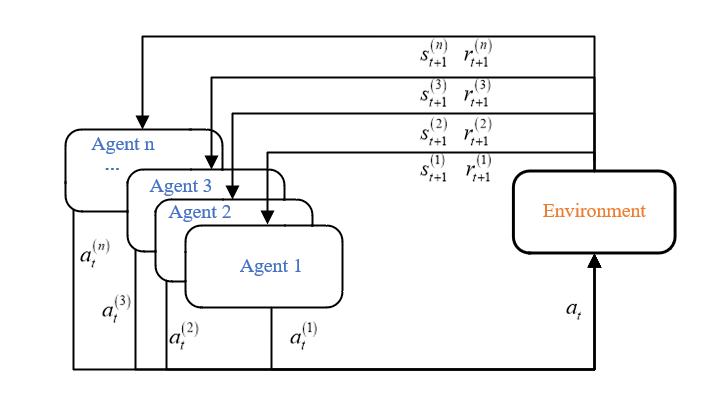
\includegraphics[scale=0.66]{images/multi_agent.png}
    \caption{Progression of a multi-agent reinforcement learning problem}
    \label{fig:multi_agent}
\end{figure*}


\subsection{Experiment Setting}
\label{sec:experiment}

We plan to carry out three major case studies with the simulation environment BlueSky to demonstrate the effectiveness of the D2MARL method. In the three case study listed below, the construction of the virtual sector, intersections,routes and aircraft are all the same. What we change and focus on is the action space.

\subsubsection{Basic Experiment: Action Space With Speed Change Only}

We try to extract the most important behaviors of the aircraft in collision avoidance, we first define the action space mainly based on the changes of the speed:

$$
A_t = \{a_-, 0, a_+\}
$$

Here $A_t$ describes the action an aircraft can take at time $t$. Then $a_-$ is to decrease the speed while $a_+$ is to increase the speed. We use $0$ to represent the action to hold the speed as the corresponding acceraltion equals zero. This means that they should reach the corresponding speed at the next time stamp, which is $v_{t+1}=\{v_{min},v_{t},v_{max}\}$. The speed we use here follow relevant regulations: $v_{min}$ is the minimum allowed cruise speed, $v_{t}$ is the current speed of the aircraft, and $v_{max}$ is the maximum allowed cruise speed. Note that the flight time is divided into several periods, and we allow $\Delta t$ for the plane to take reaction and reach the target speed.

\subsubsection{Route Relaxation: Introduce Direction Change to Actions}

Here we try to make relaxation for an aircraft's route and no longer require the plane to fly along the airlines. We allow the plane to change its flying direction as long as it remain itself inside the airway. This will bring much complexity as the track of the aircraft is on a band rather than along a line. We will allow the aircraft to choose one in three directions:

$$
A_t = \{-\pi / 12, 0, \pi / 12\}
$$

This means that within a time stamp $\Delta t$, the aircraft should be able to turn left or right for 15 degrees.

\subsubsection{Velocity Changes: Combination of Speed and Direction}

In this experiment we will introduce a more complicated action space, that is to allow the aircraft to "truly change its velocity". Considering the fact that in collision avoidance, a plane could have more flexibitity to change its velocity, and that velocity is rather a vector than a scalar, this experiment will be closer to the reality. Combined the first and the second experiment, the action space can be discretized into $3 \times 3 = 9$ actions.

